%!TEX program = xelatex

\documentclass{progartcn}
\usepackage{graphicx}
\usepackage[dvipsnames]{xcolor}
\usepackage{wrapfig}
\usepackage{enumerate}
\usepackage{amsmath,mathrsfs,amsfonts}
\usepackage{booktabs}
\usepackage{tabularx}
\usepackage{colortbl}
\usepackage{multirow,makecell}
\usepackage{multicol}
\usepackage{ulem} % \uline
\usepackage{listings}
\usepackage{tikz}
\usepackage{tcolorbox}
\usepackage{fontawesome}


\title{\bfseries\sffamily
  计算机系统结构实验3 \\ 简单的类 MIPS 单周期处理器功能部件的设计与实现(一)
}
\author{胡晨志 521021910107}
\date{}


\begin{document}

\sloppy % 解决中英文混排文字超出边界问题


\maketitle
\thispagestyle{empty}

\begin{abstract}
\noindent 在lab03中,我继续学习Verilog语言并实现了主控制单元、ALU控制单元和ALU等功能,为后续搭建单周期处理器和流水线作准备。

\vspace{2ex}
\noindent \textbf{关键字:}Vivado,\hspace{.5em}Verilog
\end{abstract}

\tableofcontents

\setcounter{page}{0}
\newpage

\section{实验目的}

\begin{itemize}
  \item 理解主控制部件或单元、ALU控制器单元、ALU单元的原理
  \item 熟悉所需的Mips指令集
  \item 使用 Verilog HD 设计与实现主控制器部件(Ctr)
  \item 使用 Verilog 设计与实现 ALU 控制器部件(ALUCtr)
  \item ALU 功能部件的实现
  \item 使用 Vivado 进行功能模块的行为仿真
\end{itemize}

\section{原理分析}

\subsection{Vivado 工程的基本组成}

Vivado 工程的基本组成如下:

\begin{itemize}
  \item design source .v 文件:\verb|Ctr.v|,\verb|ALU.v|,\verb|ALUCtr.v|
  \item simulation source .v 文件:\verb|Ctr_tb.v|,A\verb|LU_tb.v|,\verb|ALUCtr_tb.v|
\end{itemize}

\subsection{实现原理}

按照实验指导书中所给出的真值表编写模块即可

\section{功能实现}

基于上述即可完成主控制模块的功能。三个模块的代码分别如 </>CODE \ref{cd:1},</>CODE \ref{cd:2},</>CODE \ref{cd:3} 所示。

\begin{lstlisting}[language=verilog,caption={Ctr.v},label={cd:1}]
`timescale 1ns / 1ps 

module Ctr(
    input [5:0] OpCode,
    output RegDst,
    output ALUSrc,
    output MemToReg,
    output RegWrite,
    output MemRead,
    output MemWrite,
    output Branch,
    output [1:0] ALUOp,
    output Jump
    );
    reg regDst;
    reg aluSrc;
    reg memToReg;
    reg regWrite;
    reg memRead;
    reg memWrite;
    reg branch;
    reg [1:0] aluOp;
    reg jump;
    
    always @(OpCode)
    begin
        case(OpCode)
        6'b000000: //R type
            begin
                regDst = 1;
                aluSrc = 0;
                memToReg = 0;
                regWrite = 1;
                memRead = 0;
                memWrite = 0;
                branch = 0;
                aluOp = 2'b10;
                jump = 0;
            end
        6'b100011: //lw
            begin
                regDst = 0;
                aluSrc = 1;
                memToReg = 1;
                regWrite = 1;
                memRead = 1;
                memWrite = 0;
                branch = 0;
                aluOp = 2'b00;
                jump = 0;
            end
        6'b101011: //sw
            begin
                regDst = 0;
                aluSrc = 1;
                memToReg = 0;
                regWrite = 0;
                memRead = 0;
                memWrite = 1;
                branch = 0;
                aluOp = 2'b00;
                jump = 0;
            end
        6'b000100: //beq
            begin
                regDst = 0;
                aluSrc = 0;
                memToReg = 0;
                regWrite = 0;
                memRead = 0;
                memWrite = 0;
                branch = 1;
                aluOp = 2'b01;
                jump = 0;
            end
        6'b000010: //J
            begin
                regDst = 0;
                aluSrc = 0;
                memToReg = 0;
                regWrite = 0;
                memRead = 0;
                memWrite = 0;
                branch = 0;
                aluOp = 2'b00;
                jump = 1;
            end
        default:
            begin
                regDst = 0;
                aluSrc = 0;
                memToReg = 0;
                regWrite = 0;
                memRead = 0;
                memWrite = 0;
                branch = 0;
                aluOp = 2'b00;
                jump = 0;
            end
        endcase
    end
    assign RegDst = regDst;
    assign ALUSrc = aluSrc;
    assign MemToReg = memToReg;
    assign RegWrite = regWrite;
    assign MemRead = memRead;
    assign MemWrite = memWrite;
    assign Branch = branch;
    assign ALUOp = aluOp;
    assign Jump = jump;
endmodule
\end{lstlisting}

\begin{lstlisting}[language=verilog,caption={ALUCtr.v},label={cd:2}]
`timescale 1ns / 1ps

module ALUCtr(
    input [1:0] ALUOp,
    input [5:0] Funct,
    output [3:0] ALUCtrOut
    );
    reg [3:0] aluCtrOut;
    always @ (ALUOp or Funct)
    begin
        casex ({ALUOp, Funct})
            8'b00xxxxxx : aluCtrOut = 4'b0010;
            8'b01xxxxxx : aluCtrOut = 4'b0110;
            8'b1xxx0000 : aluCtrOut = 4'b0010;
            8'b1xxx0010 : aluCtrOut = 4'b0110;
            8'b1xxx0100 : aluCtrOut = 4'b0000;
            8'b1xxx0101 : aluCtrOut = 4'b0001;
            8'b1xxx1010 : aluCtrOut = 4'b0111;
        endcase
    end
    assign ALUCtrOut = aluCtrOut;
endmodule
\end{lstlisting}

\begin{lstlisting}[language=verilog,caption={ALU.v},label={cd:3}]
`timescale 1ns / 1ps

module ALU(
    input [31:0] Input1,
    input [31:0] Input2,
    input [3:0] ALUCtr,
    output Zero,
    output [31:0] ALURes
    );
    reg zero;
    reg [31:0] aluRes;
    
    always @ (Input1 or Input2 or ALUCtr)
    begin
        if (ALUCtr == 4'b0000) // AND
        begin
            aluRes = Input1 & Input2;
            if(aluRes == 0)
                zero = 1;
            else
                zero = 0;
        end
        else if (ALUCtr == 4'b0001) // OR
        begin
            aluRes = Input1 | Input2;
            if (aluRes == 0)
                zero = 1;
            else
                zero = 0;
        end
        else if (ALUCtr == 4'b0010) // add
        begin
            aluRes = Input1 + Input2;
            if (aluRes == 0)
                zero = 1;
            else
                zero = 0;
        end
        else if (ALUCtr == 4'b0110) // sub
        begin
            aluRes = Input1 - Input2;
            if (aluRes == 0)
                zero = 1;
            else
                zero = 0;
        end
        else if (ALUCtr == 4'b0111) // slt
        begin
            aluRes = Input2 > Input1 ? 1 : 0;
            if (aluRes == 0)
                zero = 1;
            else
                zero = 0;
        end
        else if (ALUCtr == 4'b1100) // NOR
        begin
            aluRes = ~(Input1 | Input2);
            if (aluRes == 0)
                zero = 1;
            else
                zero = 0;
        end
    end
    assign Zero = zero;
    assign ALURes = aluRes;
endmodule
\end{lstlisting}

实现上述后,生成 \verb|Ctr_tb.v| 的激励文件用以仿真测试.

\section{结果验证}

\subsection{测试用激励文件}

按照实验指导书的要求编写 \verb|Ctr_tb.v|,\verb|ALUCtr_tb.v|,\verb|ALU.v|文件,代码如 </>CODE \ref{cd:4}, </>CODE \ref{cd:5}, </>CODE \ref{cd:6}, 所示。

\begin{lstlisting}[language=verilog,caption={Ctr\_tb.v},label={cd:4}]
`timescale 1ns / 1ps

module Ctr_tb(

    );
    reg [5:0] OpCode;
    wire RegDst;
    wire ALUSrc;
    wire MemToReg;
    wire RegWrite;
    wire MemRead;
    wire MemWrite;
    wire Branch;
    wire [1:0] ALUOp;
    wire Jump;
    
    Ctr u0 (
        .OpCode(OpCode),
        .RegDst(RegDst),
        .ALUSrc(ALUSrc),
        .MemToReg(MemToReg),
        .RegWrite(RegWrite),
        .MemRead(MemRead),
        .MemWrite(MemWrite),
        .Branch(Branch),
        .ALUOp(ALUOp),
        .Jump(Jump)
    );
    
    initial begin
        // Initialize Inputs
        OpCode = 0;
        
        // Wait 100 ns for global reset to finish
        #100;
        
        #100 OpCode = 6'b000000;//R-type
        #100 OpCode = 6'b100011;//lw
        #100 OpCode = 6'b101011;//sw
        #100 OpCode = 6'b000100;//beq
        #100 OpCode = 6'b000010;//J
        #100 OpCode = 6'b010101;
    end
endmodule
\end{lstlisting}

\begin{lstlisting}[language=verilog,caption={ALUCtr\_tb.v},label={cd:5}]
`timescale 1ns / 1ps

module ALUCtr_tb(

    );
    reg [1:0] ALUOp;
    reg [5:0] Funct;
    wire [3:0] ALUCtrOut;
    
    ALUCtr u0 (
        .ALUOp(ALUOp),
        .Funct(Funct),
        .ALUCtrOut(ALUCtrOut)
    );
    
    initial begin
        // Initialize Inputs
        ALUOp = 0;
        Funct = 0;
        
        // Wait 100 ns for global reset to finish
        #100;
        
        #50 ALUOp = 2'b00; Funct = 6'bxxxxxx;
        #50 ALUOp = 2'bx1; Funct = 6'bxxxxxx;
        #50 ALUOp = 2'b1x; Funct = 6'bxx0000;
        #50 ALUOp = 2'b1x; Funct = 6'bxx0010;
        #50 ALUOp = 2'b1x; Funct = 6'bxx0100;
        #50 ALUOp = 2'b1x; Funct = 6'bxx0101;
        #50 ALUOp = 2'b1x; Funct = 6'bxx1010;
    end
endmodule
\end{lstlisting}

\begin{lstlisting}[language=verilog,caption={ALU\_tb.v},label={cd:6}]
`timescale 1ns / 1ps

module ALU_tb(

    );
    reg [31:0] Input1;
    reg [31:0] Input2;
    reg [3:0] ALUCtr;
    wire Zero;
    wire [31:0] ALURes;
    
    ALU u0 (
        .Input1(Input1),
        .Input2(Input2),
        .ALUCtr(ALUCtr),
        .Zero(Zero),
        .ALURes(ALURes)
    );
    
    initial begin
        Input1 = 0;
        Input2 = 0;
        ALUCtr = 0;
        
        #100 ALUCtr = 4'b0000; Input1 = 15; Input2 = 10;
        #100 ALUCtr = 4'b0001; Input1 = 15; Input2 = 10;
        #100 ALUCtr = 4'b0010; Input1 = 15; Input2 = 10;
        #100 ALUCtr = 4'b0110; Input1 = 15; Input2 = 10;
        #100 ALUCtr = 4'b0110; Input1 = 10; Input2 = 15;
        #100 ALUCtr = 4'b0111; Input1 = 15; Input2 = 10;
        #100 ALUCtr = 4'b0111; Input1 = 10; Input2 = 15;
        #100 ALUCtr = 4'b1100; Input1 = 1; Input2 = 1;
        #100 ALUCtr = 4'b1100; Input1 = 16; Input2 = 1;
    end
endmodule
\end{lstlisting}

\subsection{仿真测试}

主控制单元和ALU单元仿真结果如图\ref{fig:1},\ref{fig:2},\ref{fig:3}所示。图\ref{fig:3}和图\ref{fig:4}展示了ALU控制单元的两种不同波形,区别在于\verb|ALUCtr_tb.v|,前者的代码如 </> CODE \ref{cd:5} 所示,后者将前者代码中的所有 x 置为0即可.

\begin{figure}[htbp]
    %是可选项 h表示的是here在这里插入,t表示的是在页面的顶部插入
    \centering
    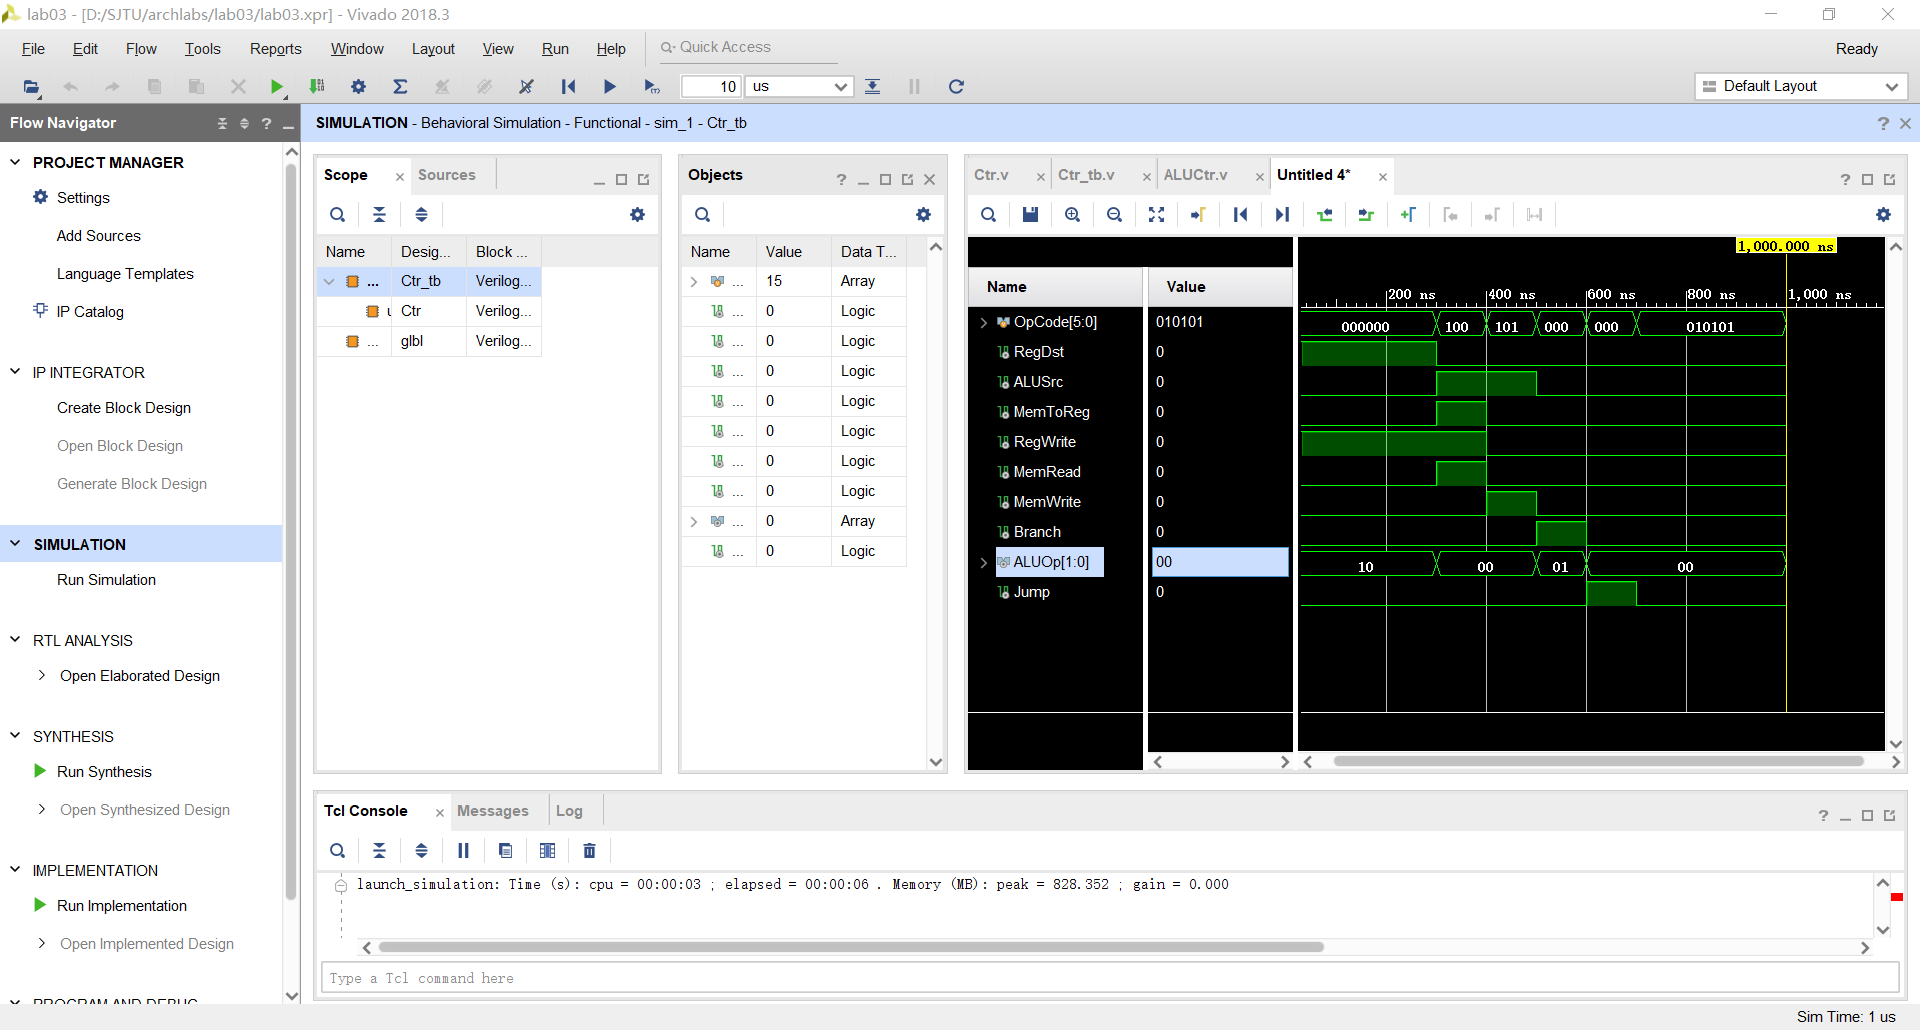
\includegraphics[scale=0.3]{../figure/03/lab03-1.PNG}
    \caption{主控制单元实验结果}\label{fig:1}
\end{figure}

\begin{figure}[htbp]
    %是可选项 h表示的是here在这里插入,t表示的是在页面的顶部插入
    \centering
    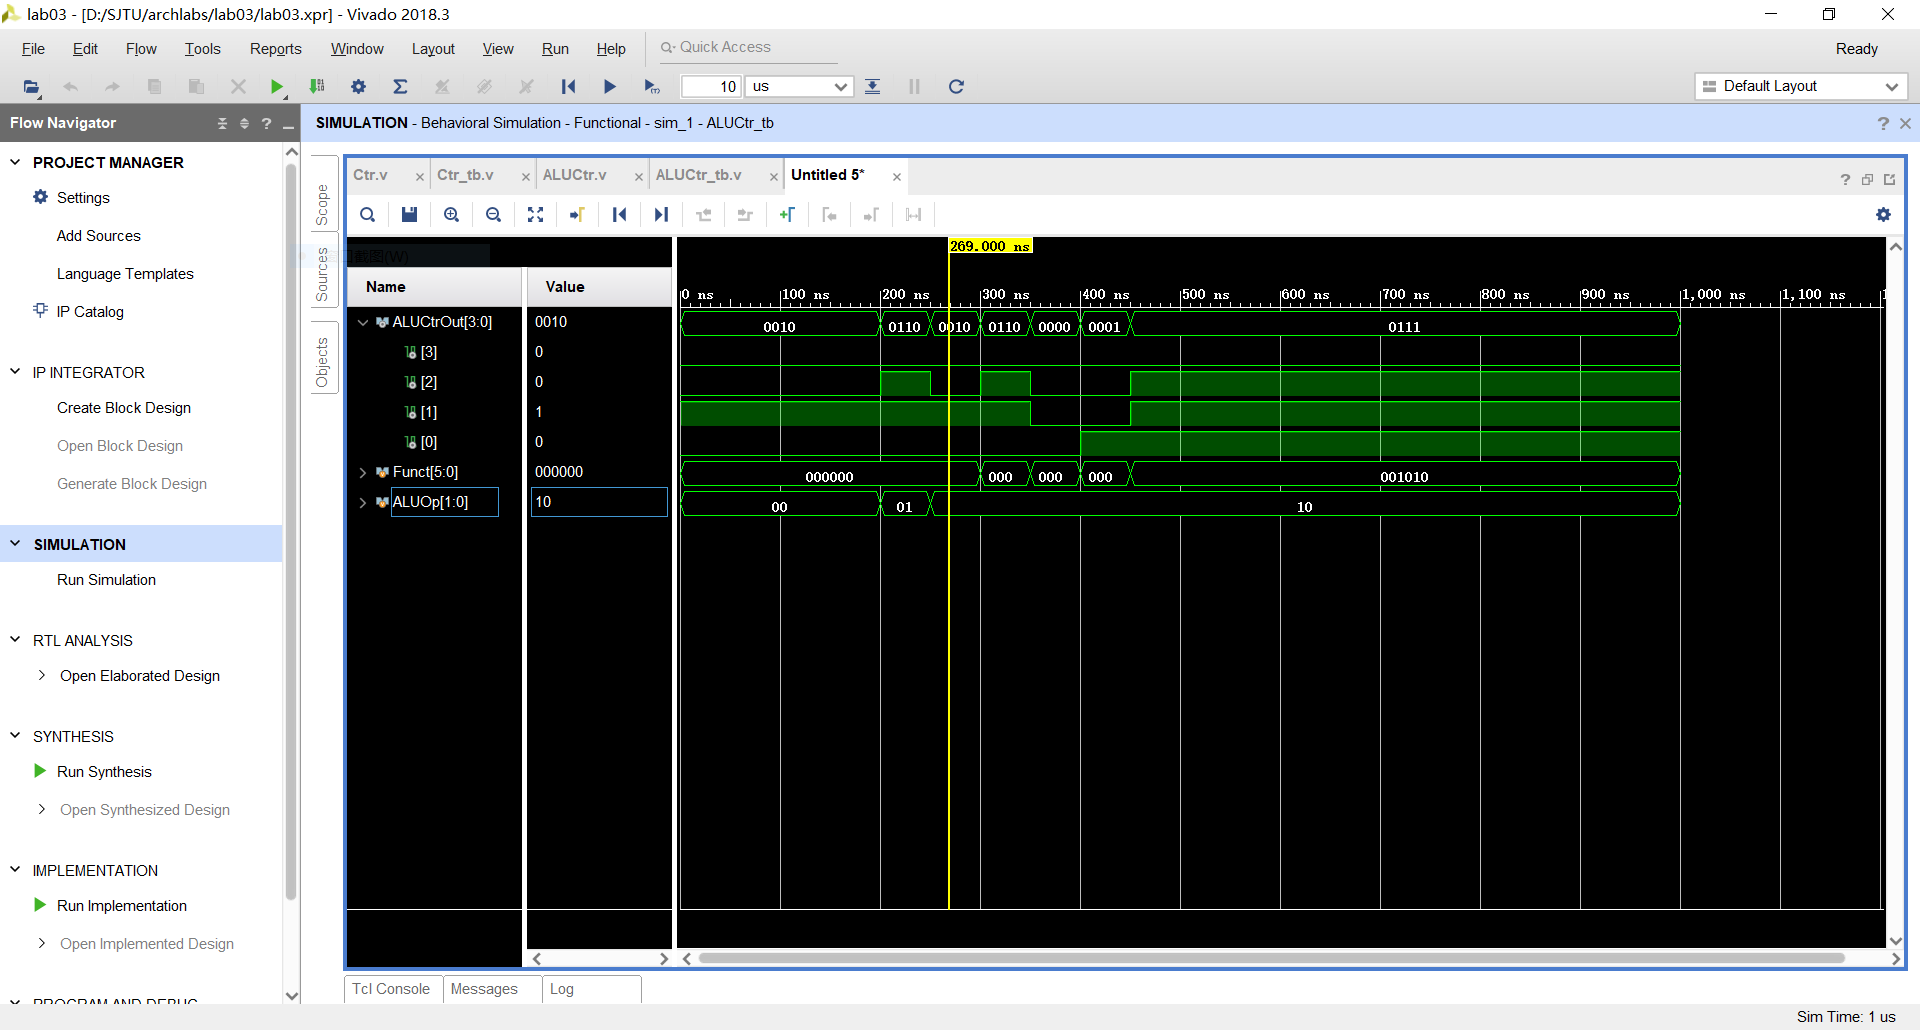
\includegraphics[scale=0.3]{../figure/03/lab03-2.PNG}
    \caption{ALU实验结果}\label{fig:2}
\end{figure}

\begin{figure}[htbp]
    %是可选项 h表示的是here在这里插入,t表示的是在页面的顶部插入
    \centering
    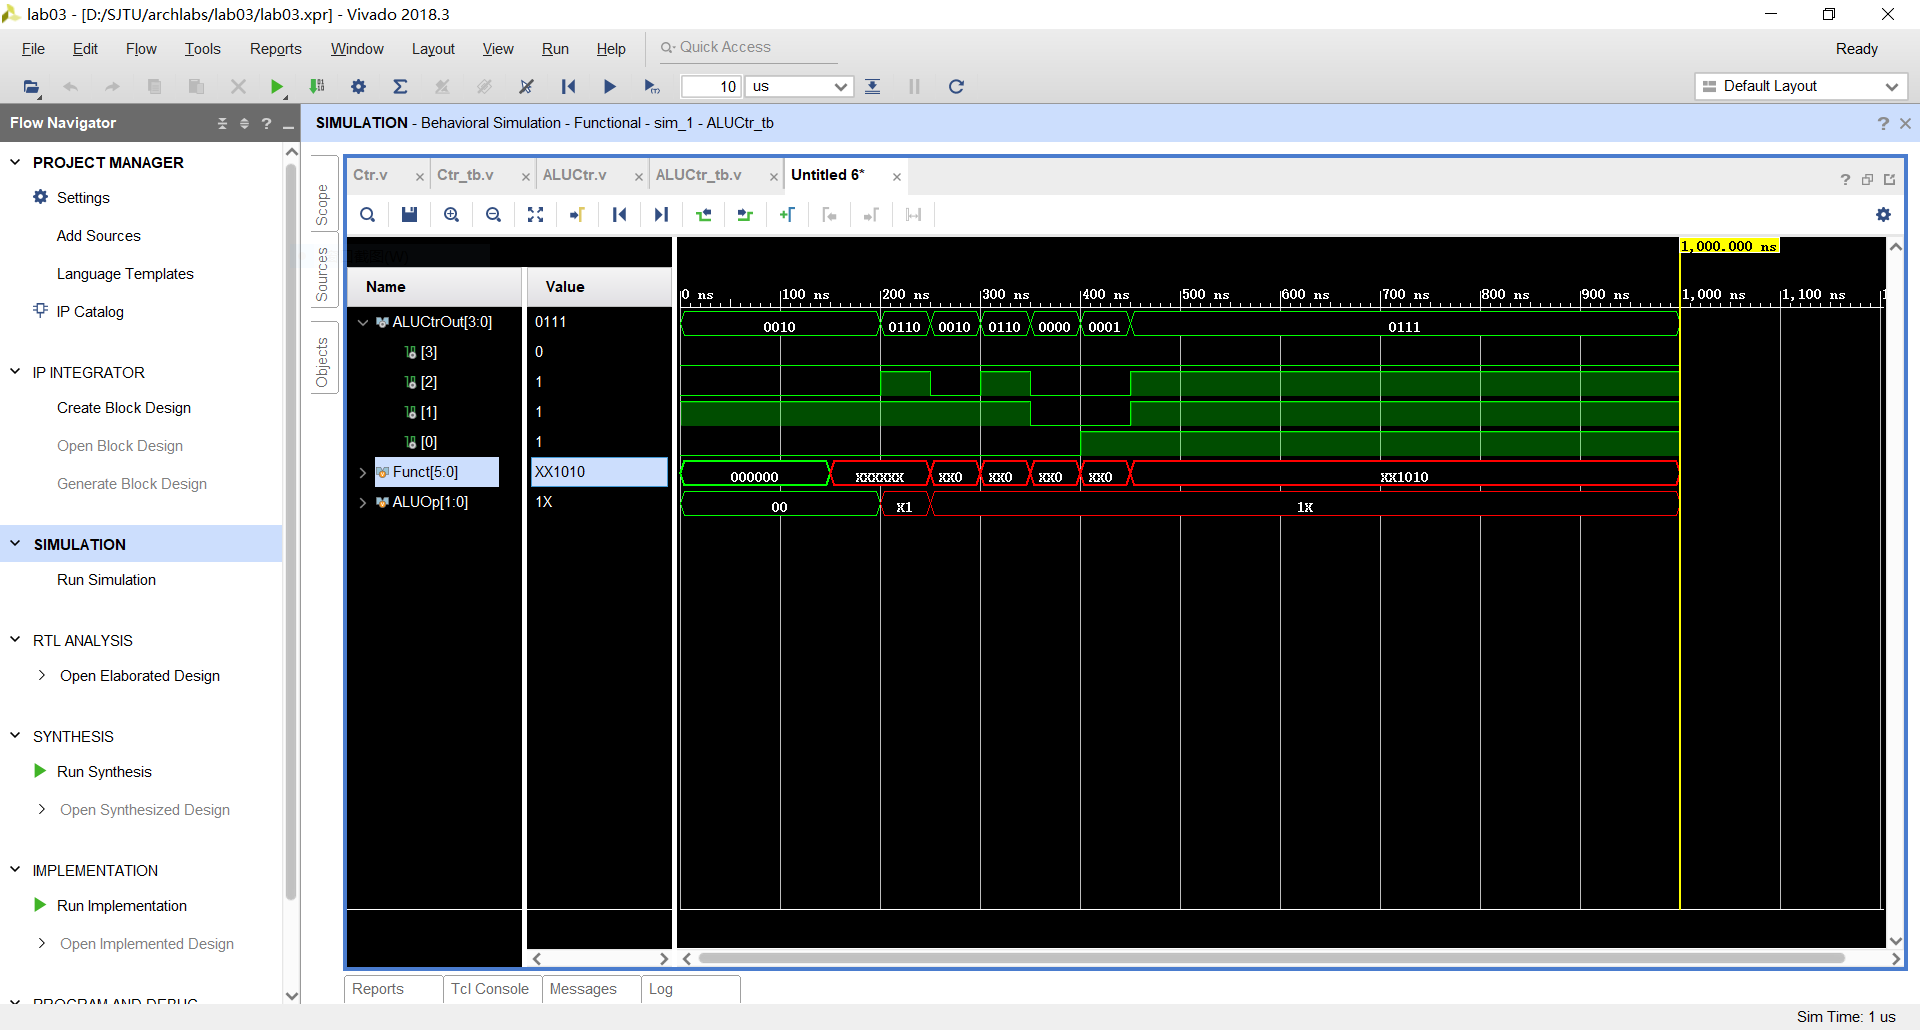
\includegraphics[scale=0.3]{../figure/03/lab03-3.PNG}
    \caption{ALU控制单元实验结果1}\label{fig:3}
\end{figure}

\begin{figure}[htbp]
    %是可选项 h表示的是here在这里插入,t表示的是在页面的顶部插入
    \centering
    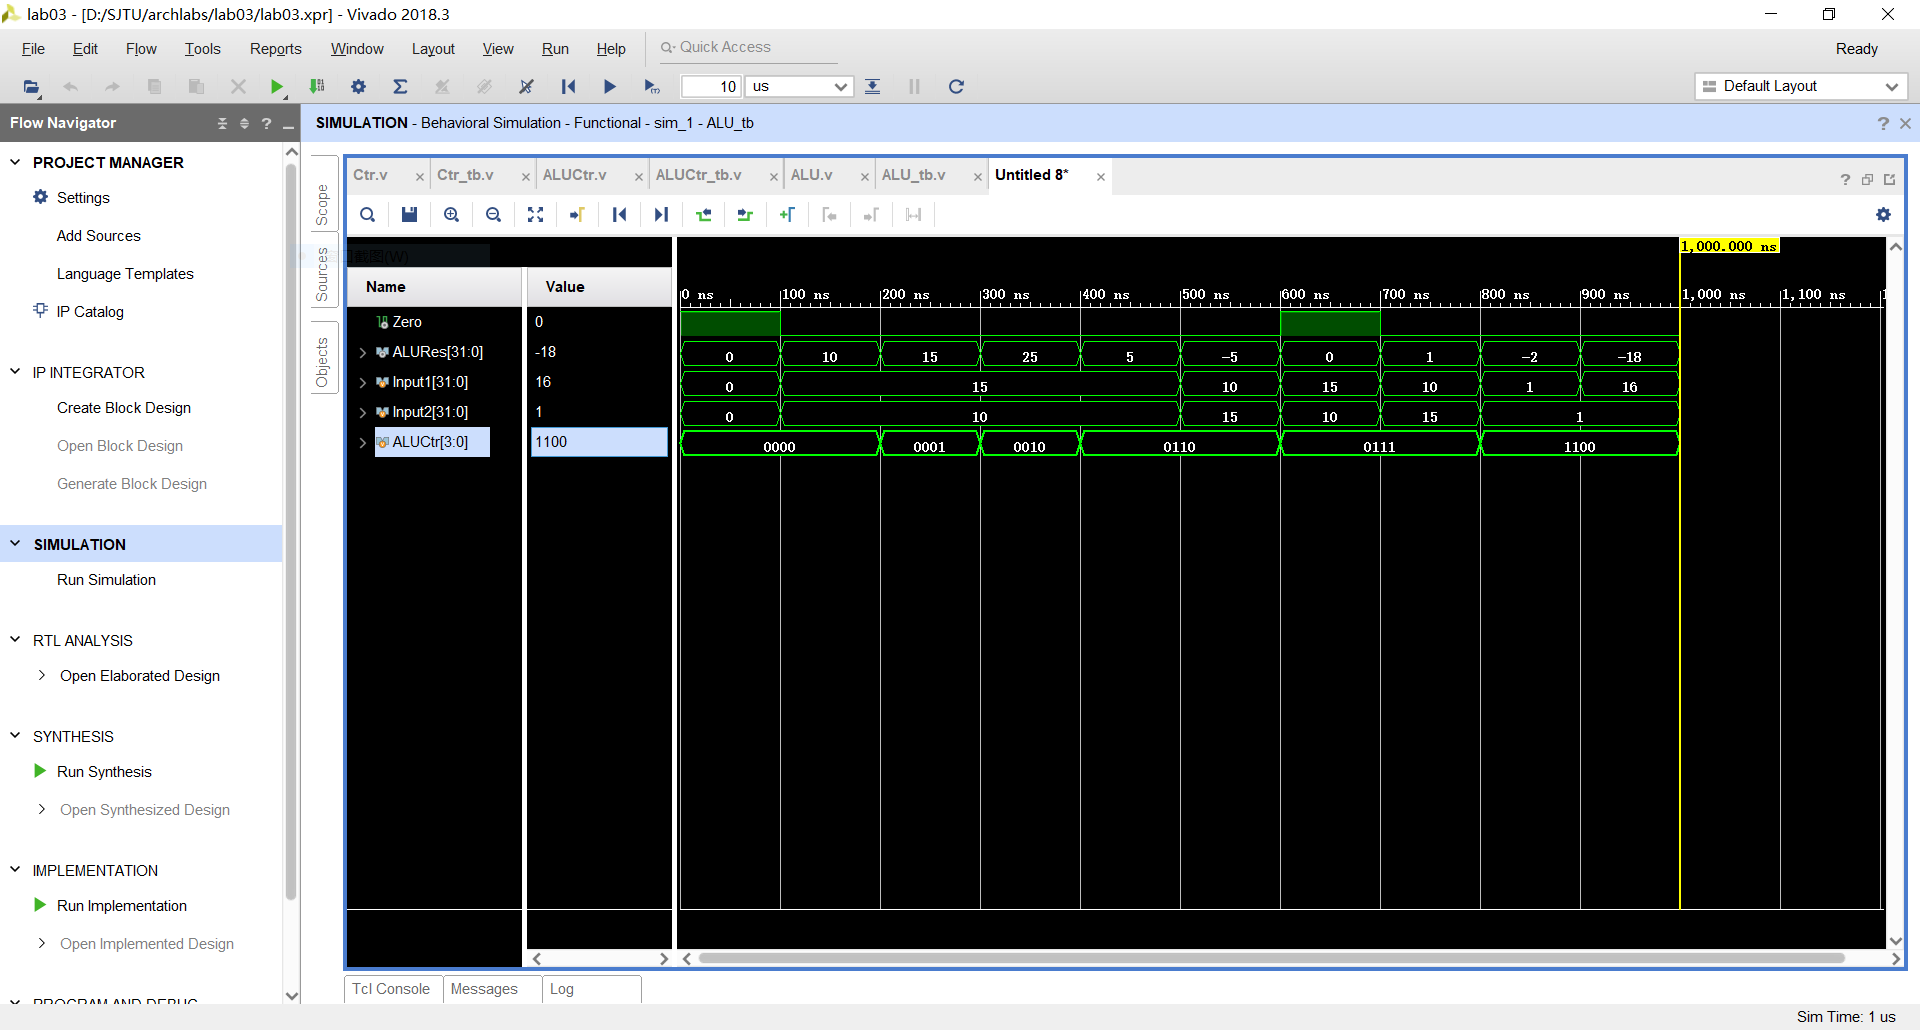
\includegraphics[scale=0.3]{../figure/03/lab03-4.PNG}
    \caption{ALU控制单元实验结果2}\label{fig:4}
\end{figure}

\section{反思与总结}

本次实验由于给出了各个模块的真值表,相对比较简单。我也通过本次实验回顾了主控制单元和ALU的相关知识。同时我也通过本次实验学习了\verb|case|,\verb|casex|的相关语法,收获良多。

\end{document}
